%\documentclass[12pt,notitlepage]{article}
\documentclass[a4paper,12pt]{article}
\usepackage[utf8]{inputenc}
\usepackage{graphicx}
\usepackage{verbatim}
\usepackage{amsthm}
\usepackage{amssymb}
\usepackage{pdfpages}
\usepackage{amsmath}
\usepackage{tikzsymbols}
\usepackage{mathtools}
\DeclarePairedDelimiter\ceil{\lceil}{\rceil}
\DeclarePairedDelimiter\floor{\lfloor}{\rfloor}

\usepackage{hyperref}
%\usepackage[T1]{fontenc}
\usepackage{url}
\usepackage{lipsum}
\usepackage{array}
\usepackage{multirow}
\usepackage{float}
\usepackage{lscape}
\usepackage{colortbl}
\newcolumntype{P}[1]{>{\centering\arraybackslash}p{#1}}
\usepackage[nottoc,numbib]{tocbibind}
\usepackage{fancyhdr}
\usepackage{hhline}
\usepackage[printonlyused]{acronym}

%\usepackage{txfonts}
\usepackage{lipsum,etoolbox}% http://ctan.org/pkg/{lipsum,etoolbox}
\usepackage{caption}
\usepackage{subcaption}

\usepackage{algorithm}
\usepackage[noend]{algpseudocode}

\makeatletter
\def\BState{\State\hskip-\ALG@thistlm}
\makeatother

\usepackage{minted}

\definecolor{black}{RGB}{0,0,0}

\usepackage{fancyvrb}

\usepackage{geometry}
\geometry{
	a4paper,
	total={170mm,257mm},
	right=3cm,
	left=3.5cm,
	top=3cm,
	bottom=3cm
}

\makeatletter
\DeclareRobustCommand{\rvdots}{%
	\vbox{
		\baselineskip4\p@\lineskiplimit\z@
		\kern-\p@
		\hbox{.}\hbox{.}\hbox{.}
}}
\makeatother

\usepackage{titlesec}
\usepackage{hyperref}
\titleclass{\subsubsubsection}{straight}[\subsection]

\newcounter{subsubsubsection}[subsubsection]
\renewcommand\thesubsubsubsection{\thesubsubsection.\arabic{subsubsubsection}}
\renewcommand\theparagraph{\thesubsubsubsection.\arabic{paragraph}} % optional; useful if paragraphs are to be numbered

\titleformat{\subsubsubsection}
{\normalfont\normalsize\bfseries}{\thesubsubsubsection}{1em}{}
\titlespacing*{\subsubsubsection}
{0pt}{3.25ex plus 1ex minus .2ex}{1.5ex plus .2ex}

\makeatletter
\renewcommand\paragraph{\@startsection{paragraph}{5}{\z@}%
	{3.25ex \@plus1ex \@minus.2ex}%
	{-1em}%
	{\normalfont\normalsize\bfseries}}
\renewcommand\subparagraph{\@startsection{subparagraph}{6}{\parindent}%
	{3.25ex \@plus1ex \@minus .2ex}%
	{-1em}%
	{\normalfont\normalsize\bfseries}}
\def\toclevel@subsubsubsection{4}
\def\toclevel@paragraph{5}
\def\toclevel@paragraph{6}
\def\l@subsubsubsection{\@dottedtocline{4}{7em}{4em}}
\def\l@paragraph{\@dottedtocline{5}{10em}{5em}}
\def\l@subparagraph{\@dottedtocline{6}{14em}{6em}}
\makeatother

\setcounter{secnumdepth}{4}
\setcounter{tocdepth}{4}
\newcommand{\und}{\underline{\hspace{.10in}}}
\begin{document}
	\begin{titlepage}
		\begin{center}
			\vspace*{9em}
			\Huge 
			MH4920\\ Supervised Independent Study I\\
			\vspace*{4em}
			\LARGE
			\textbf{Environment Variable \& Set-UID\\}		
			\vspace{4em}
			\textbf{Brandon Goh Wen Heng}\\
			\vspace*{4em}
			Academic Year 2017/18
			\vfill
		\end{center}
	\end{titlepage}
	\pagenumbering{roman}
\tableofcontents
\newpage
\pagenumbering{arabic}
\section{Introduction}
Environment variables are dynamic-named variables that affects running programs on a particular system. Common environment variables include \texttt{PATH}, where it is used to locate files for execution and \texttt{TMP}, used to describe the location or folder to store temporary files.
\section{Overview}
This lab will explore the use of environment variables, the process of propagation from parent to child processes and how environment variables affect running processes in the system. In particular, we pay special attention to the use of environment variables with respect to Set-UID programs.
\newpage
\section{Lab}
\subsection{Manipulating Environment Variables}
{\par \noindent We look at the basics of environment variables, which is to firstly set, list and remove the variables.}
\begin{enumerate}
	\item To set environment variables, we use the \texttt{export} command.
	\item To list the environment variables, the commands \texttt{env | grep <env name>} or \texttt{printenv}.
	\item To remove environment variables, \texttt{unset} command is nice.
\end{enumerate}
{\par \noindent Looking in detail at the execution of this commands, the figure below lists environment variables that exists in the system by default.}
\begin{figure}[H]
	\centering
	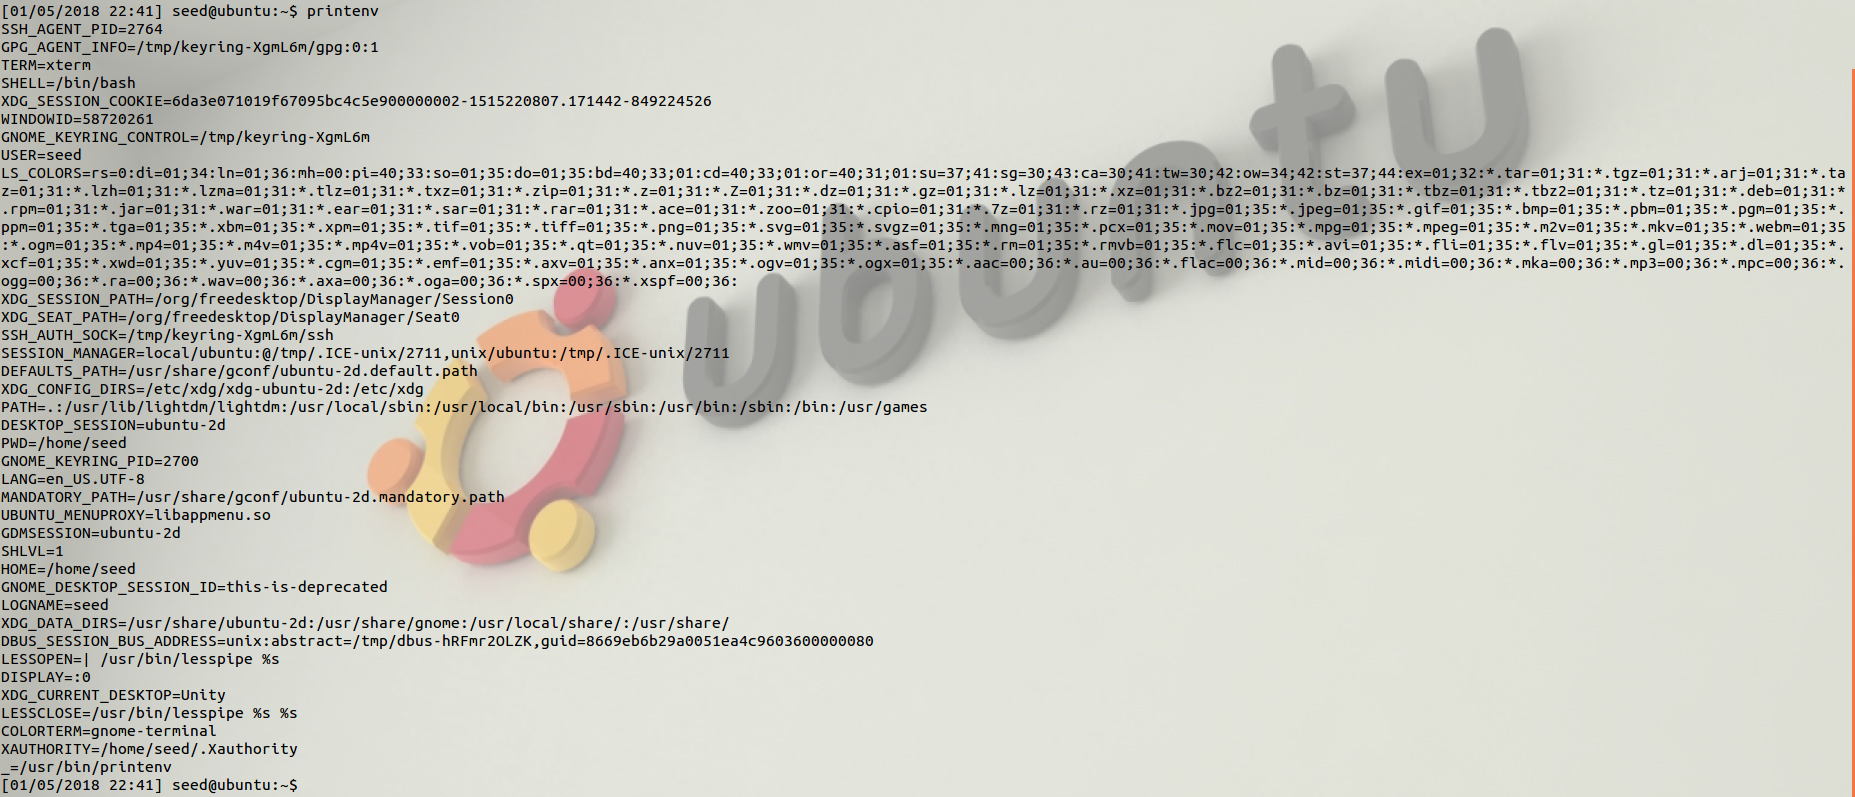
\includegraphics[width=0.95\linewidth]{ListEnv}
	\caption{Environment Variable List}
	\label{fig:listenv}
\end{figure}

{\par \noindent Environment variables can be inserted into the system using \texttt{export} where needed. In this instance, the environment variable \texttt{SOMEVAR} is set with the value \texttt{defined}. Figure 3 shows the existence of the newly defined environment variable and can now be located when we query the list of environment variables. The user-defined variable is highlighted in \text{\color{red}red}.}
\begin{figure}[H]
	\centering
	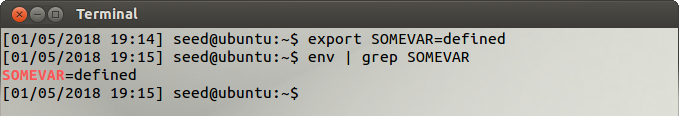
\includegraphics[width=0.9\linewidth]{VarDef}
	\caption{Defined Environment Variable}
	\label{fig:vardef}
\end{figure}
{\par \noindent Finally, removing the user-defined environment variable requires the use of the \texttt{unset} command and it will not be displayed when the \texttt{env | grep SOMEVAR} command is executed.}
\begin{figure}[H]
	\centering
	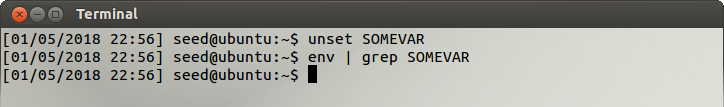
\includegraphics[width=0.9\linewidth]{VarRemoval}
	\caption{Removal of Environment Variable}
	\label{fig:varremoval}
\end{figure}

\subsection{Process Inheritance}
{\par \noindent In the current subsection, we fork the parent process to study how the environment variables affect both the parent and the child process. We also look at the inheritance properties of these processes. The \texttt{C} code that helps us to print the environment variables for the child and the parent process has been attached to the \hyperref[Appsec:3.2]{Appendix}.\\}
{\par \noindent The code below compiles the \texttt{C} code for the parent and child process separately (after toggling the respective \texttt{printenv()} lines), executes the two programs and makes use of the \texttt{diff} command to show the difference in the outputs of the environment variables of the parent and the child process.}
\begin{verbatim}
$ gcc -o childproc childprocess.c
$ gcc -o parproc parprocess.c
$ parproc > parproc.txt && childproc > childproc.txt
$ diff parproc.txt childproc.txt > diff.txt
\end{verbatim}
The output from the \texttt{diff} command only lies in the last line where it denotes the name of the file being executed. Figure 4 shows the graphical output from the terminal. This indicates that the same set of environment variables residing on the system affects both the parent and the child processes.
\begin{figure}[H]
	\centering
	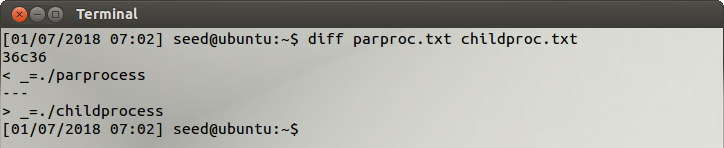
\includegraphics[width=0.9\linewidth]{NoDiffVar}
	\caption{No Difference in Environment Variables}
	\label{fig:nodiffvar}
\end{figure}
\subsection{Execution of \texttt{execve()}}
{\par \noindent The \texttt{execve()} command is analysed in this subsection, to determine whether the execution of the program is affected by the environment variables. The \texttt{C} code that will be used has been attached to the \hyperref[Appsec:3.3]{Appendix}.}\\
{\par \noindent We need to first look at the function header of \texttt{execve()} and understand its function before continuing.}
\begin{verbatim}
execve(const char *filename, char *const argv[], 
char *const envp[]);
\end{verbatim}
The first parameter is the file to be executed or the command name, while the second parameter will include the parameters for the executed file. The last parameter will include the environment variables that may be used by the program during execution with the form \textit{Name=Value}. If there are no environment variables to be included in the execution of the program, ``\texttt{NULL}'' is used.\\\\
When executing the \texttt{C} program with the following line,
\begin{verbatim}
execve("/usr/bin/env", argv, NULL);
\end{verbatim}
there is no output from the program. This is due to the existence of \texttt{NULL} in the third parameter of the function. When \texttt{NULL} is used, no environment variables are passed when calling the \texttt{env} function and therefore there are no environment variables for output.\\
\begin{figure}[H]
	\centering
	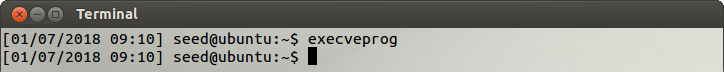
\includegraphics[width=0.9\linewidth]{execveNULL}
	\caption{\texttt{NULL} in \texttt{execve}}
	\label{fig:execvenull}
\end{figure}
{\par \noindent The third parameter is now changed from \texttt{NULL} to \texttt{environ}, i.e. 
\begin{verbatim}execve("/usr/bin/env", argv, environ);\end{verbatim} 
Execution of this compiled program now shows all the environment variables. \texttt{environ} is used to list all the environment variables in the user environment. As this is passed to the \texttt{env} function, execution will now output all the environment variables in the user environment.}
\begin{figure}[H]
	\centering
	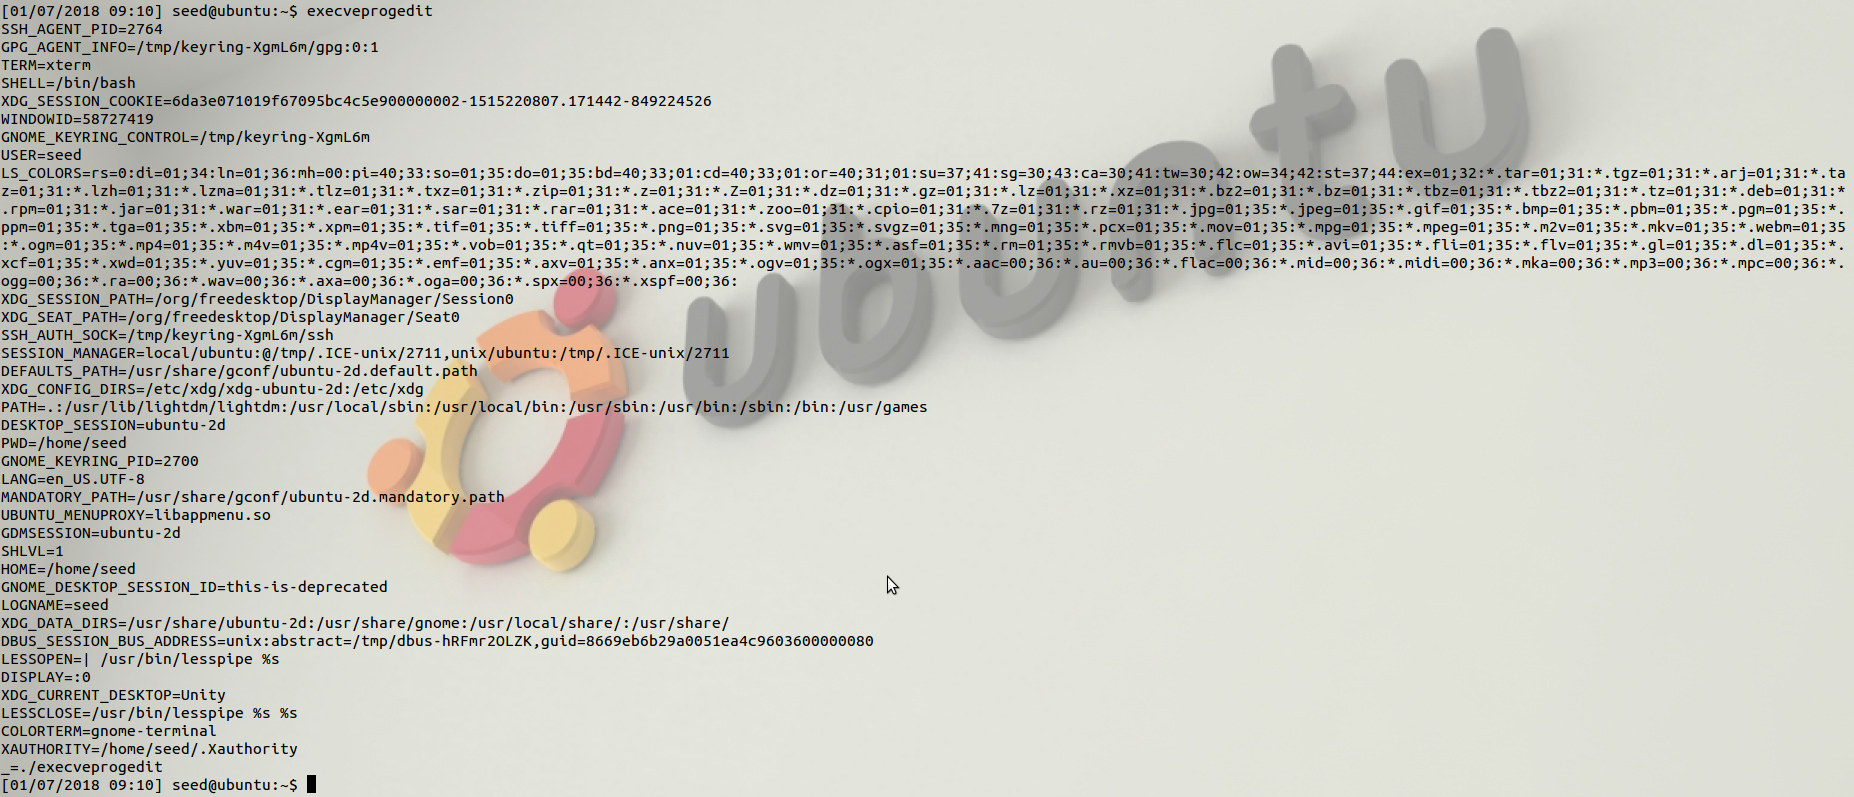
\includegraphics[width=0.95\linewidth]{execveenviron}
	\caption{\texttt{environ} in \texttt{execve}}
	\label{fig:execveenviron}
\end{figure}
\subsection{Execution of \texttt{system()}}
In this subsection, we focus on calling the \texttt{system} function and observe how environment variables are passed. When \texttt{system} is called, \texttt{execl} is executed and the command is passed as one of the parameters. Since \texttt{execl} does not have the parameter where \texttt{const char* envp[]} can be explicitly defined, the variable \texttt{environ} will be used instead. These will be used as the parameters when executing \texttt{execve} and therefore the execution of the code will show all environment variables. The \texttt{C} code used to output the environment variables using \texttt{system} is attached in the \hyperref[Appsec:3.4]{Appendix}.
\begin{figure}[H]
	\centering
	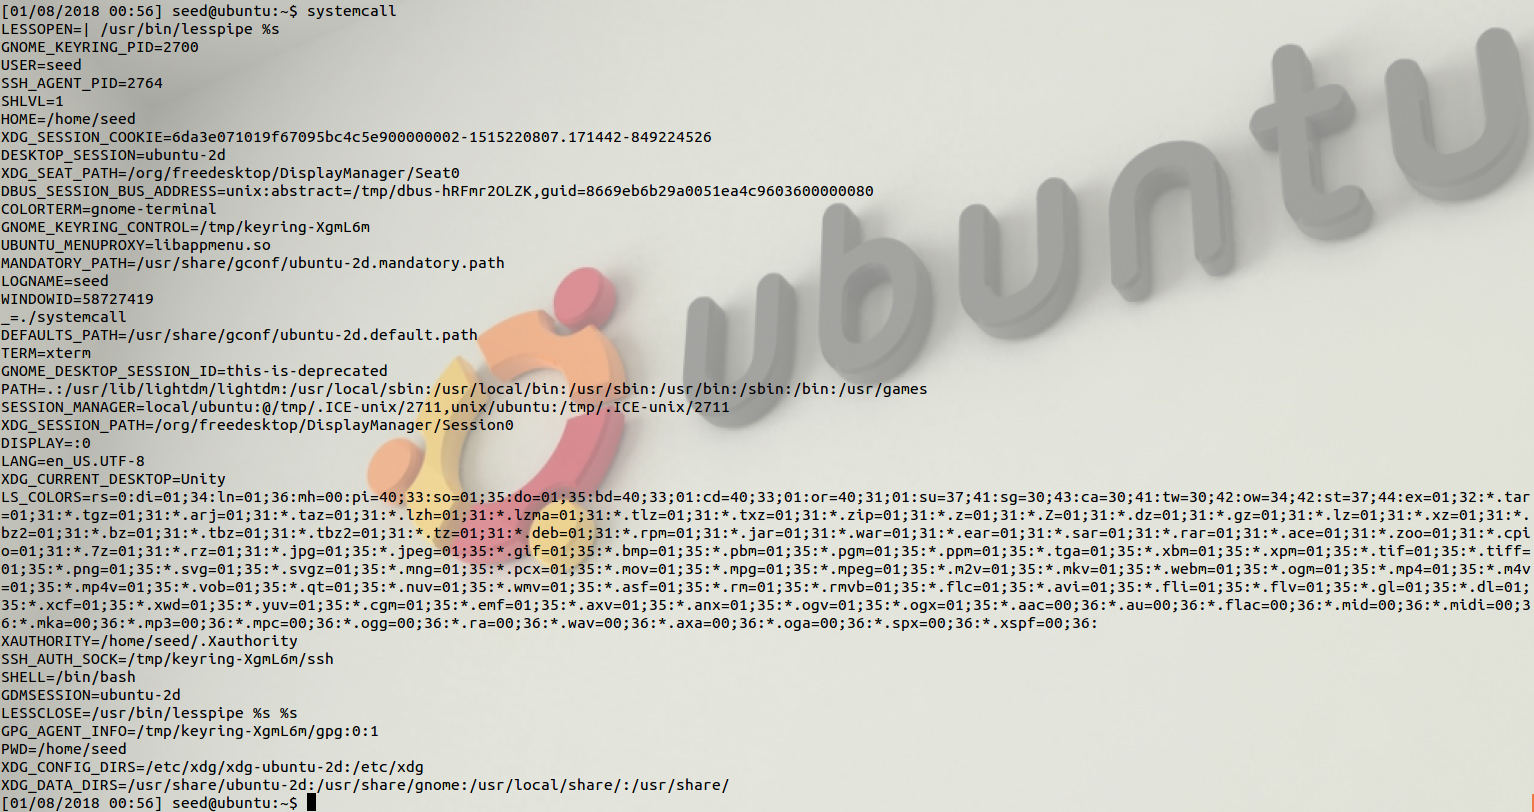
\includegraphics[width=0.95\linewidth]{systemcall}
	\caption{\texttt{system} execution}
	\label{fig:systemcall}
\end{figure}
\subsection{Environment Variables \& \texttt{Set-UID} Programs}
\texttt{Set-UID} is an important security feature in Unix systems. In this subsection, it is important to understand how \texttt{Set-UID} programs are affected by environment variables and the user's process.\\\\To begin, a \texttt{C} program is created to print out all the environment variables in the current process. The \texttt{C} code has been attached in the \hyperref[Appsec:3.5]{Appendix} for reference. Assuming that the program name is \textit{setuid}, we use the following commands to make root the owner of the \texttt{Set-UID} program.
\begin{verbatim}
$ su
# gcc -o setuid setuid.c
# chmod 4755 setuid
$ exit
\end{verbatim}
To examine if the \texttt{Set-UID} program is affected by the user's process, we add three environment variables using the user account (not root).
\begin{verbatim}
$ export PATH=/home/seed/lab:$PATH
$ export LD_LIBRARY_PATH=/home/seed/lib
$ export NEWENV=var
\end{verbatim}
As \texttt{PATH} already exists in the system, \texttt{:\$PATH} is added to the back to ensure that the existing \texttt{PATH} value is concatenated to the back of the newly added value.\\\\Execution of the \texttt{Set-UID} programs shows that the edited \texttt{PATH} and \texttt{NEWENV} are displayed in the output. The \texttt{LD\_LIBRARY\_PATH} is however not in the list of environment variables when the \texttt{Set-UID} program is being run. As \texttt{LD\_LIBRARY\_PATH} can be used to run malicious libraries, it is ignored by default if it is a \texttt{Set-UID} program. Figure 8 and 9 shows the difference in the user environments between a \texttt{Set-UID} and a non \texttt{Set-UID} program.
\begin{figure}[!h]
	\centering
	\begin{minipage}{0.5\linewidth}
		\centering
		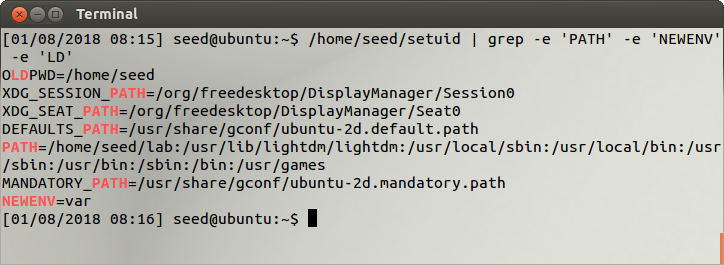
\includegraphics[width=0.98\linewidth]{setuidenvvar}
		\caption{\texttt{Set-UID} program}
		\label{fig:setuidenvvar}
	\end{minipage}%
	\begin{minipage}{0.5\linewidth}
		\centering
		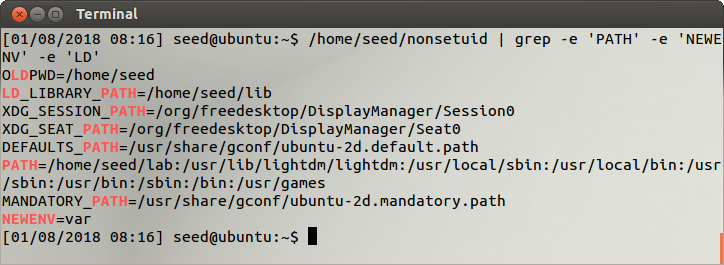
\includegraphics[width=0.98\linewidth]{nonsetuidenvvar}
		\caption{Non \texttt{Set-UID} program}
		\label{fig:nonsetuidenvvar}
	\end{minipage}
\end{figure}
\subsection{\texttt{PATH} Environment Variable \& \texttt{Set-UID}}
Using \texttt{system} as a \texttt{Set-UID} program is dangerous as the \texttt{PATH} environment variable can be exploited to run malicious code. In this subsection, we will explore the use of the \texttt{PATH} environment variable and the interaction with the \texttt{Set-UID} program.\\\\A \texttt{Set-UID} program written in \texttt{C} is defined such that it uses the \texttt{system} command to execute \texttt{ls}. The program is  compiled with the name \textit{setuidpath} for readability purposes and the code can be referenced in the \hyperref[Appsec:3.6]{Appendix}. The \texttt{PATH} environment variable is now edited to point to another directory and placed at the front. Placing the directory at the front ensures that the program will always look into our added directory first before moving on to the following directories in the list to find the respective program to be executed. In this instance, we run the following code to update \texttt{PATH},
\begin{verbatim}$ export PATH=/home/seed:$PATH\end{verbatim}
We create a file that calls \texttt{sh} using system. The code has also been attached in the \hyperref[Appsec:3.6.2]{Appendix}. The following line of code is run to ensure that the code is being compiled into a program with the name \texttt{ls} in the directory \texttt{/home/seed} that was just added.
\begin{verbatim}
$ gcc -o ls callsh.c
\end{verbatim}
When \textit{setuidpath} is run, a shell is obtained as the process that calls the shell is privileged. Further scripting reveals that we have obtained root access to the system using a \texttt{Set-UID} program.
\begin{figure}[h]
	\centering
	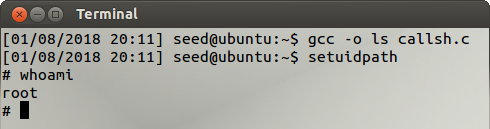
\includegraphics[width=0.9\linewidth]{PATHexploit}
	\caption{Exploit using \texttt{PATH}}
	\label{fig:pathexploit}
\end{figure}
\\The results of this subsection proves that it is extremely dangerous when a \texttt{Set-UID} program uses the \texttt{system} command. It has also been shown that the \texttt{PATH} environment variable can be easily edited by a malicious user even without root privileges. Furthermore, using a relative path further increases the risk of the system being compromised.
\subsection{\texttt{LD\_PRELOAD} Environment Variable \& \texttt{Set-UID}}
The current subsection will focus on how \texttt{Set-UID} programs interact with \texttt{LD\_}\textbf{*} environment variables, in particular \texttt{LD\_PRELOAD}. The \texttt{LD\_}\textbf{*} environment variables affect the behaviour of the dynamic loaders in Linux and \texttt{LD\_PRELOAD} specifies additional user-specified shared library directories to be loaded before using the default set of directories.\\\\
A dynamic link library is created to replace the \texttt{sleep()} function in \texttt{libc}. The code for this library is attached in the \hyperref[Appsec:3.7]{Appendix}. This is compiled and \texttt{LD\_PRELOAD} is now edited to include the newly compiled library.
\begin{verbatim}
$ gcc -fPIC -g -c mylib.c
$ gcc -shared -o libmylib.so.1.0.1 mylib.o -lc
$ export LD_PRELOAD=./libmylib.so.1.0.1
\end{verbatim}
The \texttt{-fPIC} argument is used to ensure that the code generated is independent of the virtual address. Using \texttt{PIC} instead of \texttt{pic} ensures that the code generated is platform independent.\\\\A new program \textit{myprog} is created to execute the \texttt{sleep} function. The code for this simple program can be referenced from the \hyperref[Appsec:3.7.2]{Appendix}. When \textit{myprog} is run under the following circumstances, the results obtained were different.
\begin{enumerate}
	\item Running \textit{myprog} as a regular program and executing as a normal user, the string ``I am not sleeping!'' is displayed, which is expected as the sleep function in our user-defined library is used due to reading of the \texttt{LD\_PRELOAD} environment variable.
	\item Running \textit{myprog} as a \texttt{Set-UID} program and running it with a normal user will result in the program going to sleep for 5 seconds. (To observe the results clearly, \texttt{sleep(1)} was amended to \texttt{sleep(5)} instead.)
	\item Running \textit{myprog} as a \texttt{Set-UID} program and exporting the \texttt{LD\_PRELOAD} environment variable under the root account results in the string being displayed. Due to the security loophole of \texttt{LD\_PRELOAD}, the user-defined library is only loaded if the environment variable was exported with root and the program run with root.
	\item Setting \textit{myprog} as a user1 \texttt{Set-UID} program with \texttt{LD\_PRELOAD} environment variable set under user2 and executing it results in the program going to sleep for 5 seconds.
\end{enumerate}
We analyse the results obtained from the four different conditions and notice that the \texttt{LD\_PRELOAD} is ignored if the owner and the user executing the program is different, then there will be no execution of the user-defined library.
\subsection{Invoking External Programs using \texttt{system()} Versus \texttt{execve()}}
This section looks at using \texttt{system()} and \texttt{execve()} at executing external programs that are not intended. The \texttt{C} code that will be used limits the user to using the \texttt{cat} function. Due to this, the owner assumes that the user will cannot execute any write function on the system and will not be able to edit any file. The \texttt{C} code for this has been attached in the \hyperref[Appsec:3.8]{Appendix}.\\\\
The code is compiled as a \texttt{Set-UID} program with the name \textit{audit} and root as the owner. In particular, we note that the ``\texttt{;}'' operator can be used to initiate the next command. As such, running the program using the following code will allows us to obtain a shell.
\begin{verbatim}
$ audit "sometext.txt;/bin/sh"
\end{verbatim}
In this instance, a dummy file with the file name and extension \texttt{sometext.txt} will just act as the argument needed to execute the \texttt{cat} function before the shell can be obtained. After the shell has been obtained, system operations such as \text{rm -rf} can be performed even without being given root privileges.
\begin{figure}[h]
	\centering
	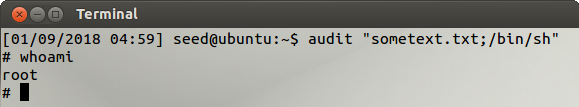
\includegraphics[width=0.9\linewidth]{systemexploit}
	\caption{Shell obtained using \texttt{system()}}
	\label{fig:systemexploit}
\end{figure}\\
When we use \texttt{execve()} instead and compile again, we note that a shell cannot be obtained this time. This is due to \texttt{execve} interpreting the entire string as an argument and hence will not be able to find the file.
\begin{figure}[h]
	\centering
	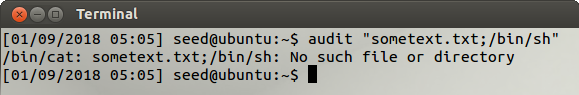
\includegraphics[width=0.9\linewidth]{execveuse}
	\caption{Cannot obtain Shell using \texttt{execve()}}
	\label{fig:execveuse}
\end{figure}

\subsection{Capability Leaking (Exploit)}
In this section, we take a look at capability leaking, where privileges are downgraded after execution but may still be accessible by non-privileged processes. Using \texttt{setuid()} sets the effective user ID of the calling process and removes root privileges if the user executing the program is not root.\\\\In the \texttt{C} code provided for \hyperref[Appsec:3.9]{this section}, a vulnerability can be found in the program where root access is revoked but the file that was previously opened under root privileges is still able to have its file edited. 
\begin{figure}[h]
	\centering
	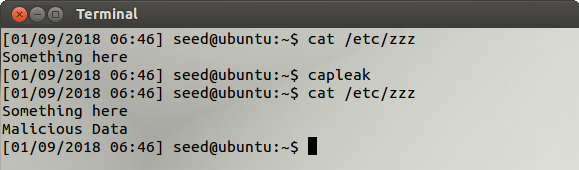
\includegraphics[width=0.9\linewidth]{capleak}
	\caption{Capability Leaking}
	\label{fig:capleak}
\end{figure}
\\In Figure 13, it can be seen that the file was successfully written as the handle that opens the file still retains root privileges and as a result is successful in writing the contents into the file even after \texttt{setuid(getuid())} has been executed.

\newpage
\addcontentsline{toc}{section}{Appendix}
\section{Appendix}
\subsection{Process Inheritance \texttt{C} Code}
\label{Appsec:3.2}

\begin{minted}{C}
#include <unistd.h>
#include <stdio.h>
#include <stdlib.h>

extern char **environ;
void printenv()
{
    int i=0;
    while (environ[i] !=NULL)
    {
        printf("%s\n", environ[i]);
        i++;
    }
}

void main()
{
    pid_t childPid;
    switch(childPid=fork())
    {
        case 0:
            printenv(); /*Child process*/
            exit(0);
        default:
            //printenv(); /*Parent process*/
            exit(0);
    }
}
\end{minted}
\newpage

\subsection{Execution of \texttt{execve()}}
\label{Appsec:3.3}
\begin{minted}{C}
#include <stdio.h>
#include <stdlib.h>

extern char **environ;

int main()
{
    char *argv[2];
    
    argv[0] = "/usr/bin/env";
    argv[1] = NULL;
    
    execve("/usr/bin/env", argv, NULL);
    
    return 0;
}
\end{minted}
\subsection{Execution of \texttt{system()}}
\label{Appsec:3.4}
\begin{minted}{C}
#include <stdio.h>
#include <stdlib.h>

int main()
{
    system("/usr/bin/env");

    return 0;
}
\end{minted}
\subsection{Envrionment Variables \& \texttt{Set-UID} Programs}
\label{Appsec:3.5}
\begin{minted}{C}
#include <stdio.h>
#include <stdlib.h>

extern char **environ;

void main()
{
    int i=0;
    while (environ[i] != NULL) {
        printf("%s\n", environ[i]);
        i++;
    }
}
\end{minted}
\subsection{\texttt{PATH} Environment Variable \& \texttt{Set-UID}}
\label{Appsec:3.6}
\begin{minted}{C}
int main()
{
    system("ls");
    return 0;
}
\end{minted}
\subsection{Call Shell}
\label{Appsec:3.6.2}
		\begin{minted}{C}
int main()
{
    system("sh");
    return 0;
}
\end{minted}
\subsection{\texttt{sleep()} Library}
\label{Appsec:3.7}
\begin{minted}{C}
#include <stdio.h>

void sleep (int s)
{
    printf("I am not sleeping!\n");
}
\end{minted}
\subsection{Execute \texttt{sleep()} Function}
\begin{minted}{C}
int main()
{
    sleep(1);
    return 0;
}
\end{minted}
\newpage
\subsection{Invoking External Programs using \texttt{system()} Versus \texttt{execve()}}
\label{Appsec:3.8}
\begin{minted}{C}
#include <string.h>
#include <stdio.h>
#include <stdlib.h>

int main(int argc, char *argv[])
{
    char *v[3];
    char *command;
    
    if (argc < 2) {
        printf("Please type a file name.\n");
        return 1;
    }
    
    v[0]="/bin/cat";
    v[1]=argv[1];
    v[2]=NULL;
    
    command = malloc(strlen(v[0]) + strlen(v[1]) + 2);
    
    sprintf(command, "%s %s", v[0], v[1]);
    
    system(command);
    //execve(v[0], v, NULL);
    
    return 0;
}
\end{minted}
\newpage
\subsection{Capability Leaking}
\label{Appsec:3.9}
\begin{minted}{C}
#include <stdio.h>
#include <stdlib.h>
#include <fcntl.h>

void main()
{
    int fd;
    fd = open("/etc/zzz", O_RDWR | O_APPEND);
    if (fd==-1) {
        printf("Cannot open /etc/zzz\n");
        exit(0);
    }
    
    sleep(1);
    
    setuid(getuid());
    
    if (fork()){
        close (fd);
        exit(0);
    } else {
    write(fd, "Malicious Data\n", 15);
    close (fd);
    }
}
\end{minted}
\end{document}